\documentclass[tikz,border=6pt]{standalone}
\usepackage[T1]{fontenc}
\usepackage[utf8]{inputenc}
\usepackage{pgfplots}
\pgfplotsset{compat=1.18}
\begin{document}
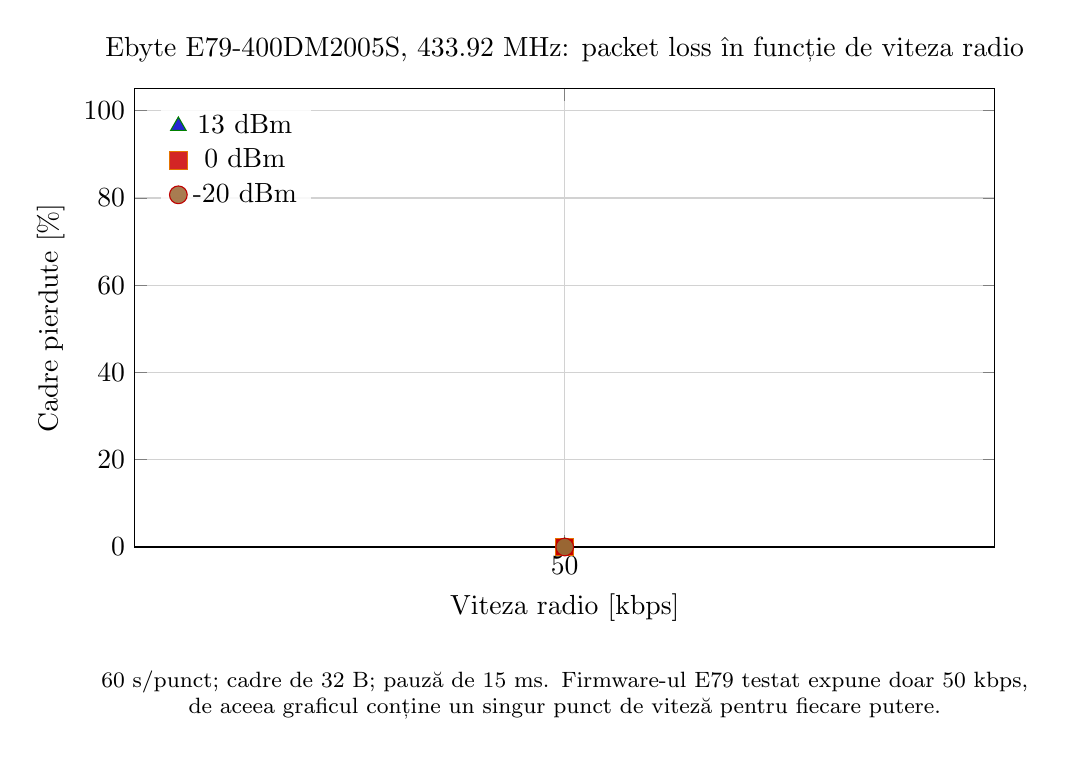
\begin{tikzpicture}
\begin{axis}[width=12.5cm, height=7.4cm,
  title={Ebyte E79-400DM2005S, 433.92 MHz: packet loss în funcție de viteza radio},
  xmin=40, xmax=60,
  xtick={50}, xticklabels={50},
  ymin=0, ymax=105, ytick={0,20,40,60,80,100},
  xlabel={Viteza radio [kbps]}, ylabel={Cadre pierdute [\%]},
  grid=both, minor grid style={gray!15}, major grid style={gray!35},
  every axis plot/.append style={only marks, mark size=3.2pt},
  legend style={draw=none, fill=white, fill opacity=0.85, text opacity=1,
    at={(0.03,0.97)}, anchor=north west, legend columns=1},
]
\addplot+[green!50!black, mark=triangle*] coordinates {(50,0)};
\addlegendentry{13 dBm}
\addplot+[orange!90!black, mark=square*] coordinates {(50,0)};
\addlegendentry{0 dBm}
\addplot+[red!75!black, mark=*] coordinates {(50,0)};
\addlegendentry{-20 dBm}
\end{axis}
\node[font=\footnotesize, align=center, text width=12cm, anchor=north]
  at ([yshift=-1.45cm]current axis.south)
  {60 s/punct; cadre de 32 B; pauză de 15 ms. Firmware-ul E79 testat expune doar 50 kbps,\\
   de aceea graficul conține un singur punct de viteză pentru fiecare putere.};
\end{tikzpicture}
\end{document}
